\section{Grafos bipartitos}
\label{sec:grafos_bipartitos}

Un grafo es \concept{bipartito} si sus vértices pueden dividirse en dos conjuntos \(X\) y \(Y\) tal que \emph{todos} los arcos del grafo tienen un extremo en \(X\) y otro en \(Y\). Formalmente:

\begin{definicion}{Grafo bipartito}{grafo_bipartito}
  Un grafo \(G\) es \concept{bipartito} si existe una partición \((X, Y)\) de su conjunto de vértices tal que cada arco del grafo une un vértice de \(X\) con uno de \(Y\). Se dice entonces que \(G\) tiene una \concept{bipartición} \((X, Y)\).
\end{definicion}

Recuérdese que para que una colección de subconjuntos constituya una partición de un conjunto, los subconjuntos deben ser: no vacíos, en este caso \(X \neq \varnothing\) y \(Y \neq \varnothing\); disjuntos, en este caso \(X \cap Y = \varnothing\); y su unión total debe ser el conjunto original, \(X \cup Y = V\).

Se dibujan dos grafos bipartitos, $Q_3$ y $K_{4,4}$:
\begin{center}
  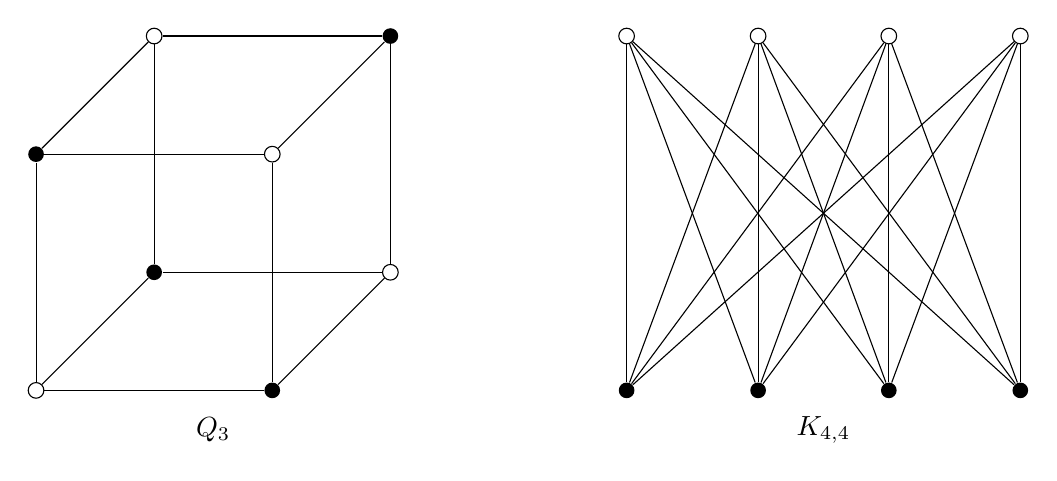
\begin{tikzpicture}[
    fvertex/.style={circle, fill=black, inner sep=2pt},
    overtex/.style={circle, draw=black, fill=white, inner sep=2pt}
  ]
    % Bipartición de Q_3: vértices con cantidad par de 1s vacíos, impares rellenos
    % x=000(open), u=010(filled), v=011(open), w=001(filled)
    % d=100(filled), a=110(open), b=111(filled), c=101(open)
    \begin{scope}
      \node[overtex] (x) at (0,   0)   {};
      \node[fvertex] (u) at (3,   0)   {};
      \node[overtex] (v) at (3,   3)   {};
      \node[fvertex] (w) at (0,   3)   {};
      \node[fvertex] (d) at (1.5, 1.5) {};
      \node[overtex] (a) at (4.5, 1.5) {};
      \node[fvertex] (b) at (4.5, 4.5) {};
      \node[overtex] (c) at (1.5, 4.5) {};
      \draw (x)--(u)--(v)--(w)--(x);
      \draw (d)--(a)--(b)--(c)--(d);
      \draw (x)--(d) (u)--(a) (v)--(b) (w)--(c);
      \node at (2.25, -0.5) {$Q_3$};
    \end{scope}
    % K_{4,4}: grafo bipartito completo
    \begin{scope}[xshift=10cm]
      \node[overtex] (t1) at (-2.5,  4.5) {};
      \node[overtex] (t2) at (-0.83, 4.5) {};
      \node[overtex] (t3) at ( 0.83, 4.5) {};
      \node[overtex] (t4) at ( 2.5,  4.5) {};
      \node[fvertex] (s1) at (-2.5,  0)   {};
      \node[fvertex] (s2) at (-0.83, 0)   {};
      \node[fvertex] (s3) at ( 0.83, 0)   {};
      \node[fvertex] (s4) at ( 2.5,  0)   {};
      \foreach \t in {t1,t2,t3,t4} {
        \foreach \s in {s1,s2,s3,s4} {
          \draw (\t)--(\s);
        }
      }
      \node at (0, -0.5) {$K_{4,4}$};
    \end{scope}
  \end{tikzpicture}
\end{center}

Si se dibuja un grafo bipartito con los vértices en \(X\) de un color y los vértices en \(Y\) de otro, no habrán vértices adyacentes del mismo color. Por eso a los grafos bipartitos se les llama \concept{grafos 2-colores}.

\subsection{Grafo completo bipartito y cota de arcos}

El grafo \concept{completo bipartito}, denotado por \(K_{m, n}\) tiene una bipartición \((X, Y)\) tal que \(|X|=m\), \(|Y|=n\). En \(K_{m,n}\) cada vértice en \(X\) está unido a todos los vértices de \(Y\), por lo cual \(\varepsilon = mn\). Naturalmente, el grafo completo bipartito tiene el máximo número de arcos de cualquier grafo bipartito.

A partir de eso se concluye que todo grafo bipartito tiene a lo sumo \(n^2/4\) arcos. Sea \(G\) un grafo con bipartición \((X, Y)\) y sea \(x=|X|\), de forma que \(n-x=|Y|\), entonces \[
\varepsilon \leq x(n-x) = nx-x^2 = n^2/4 - (n/2-x)^2 \leq n^2/4.
\] 

Sea \(C\) un ciclo en un grafo con bipartición \((X,Y)\). El vértice inicial (y final) debe estar en algún conjunto, supóngase \(X\). Los vértices de \(C\) deben estar alternadamente uno en \(X\), uno en \(Y\), uno en \(X\) y así, pues no hay arcos entre elementos de \(X\) o entre elementos de \(Y\). Eso implica que la \hyperref[sec:longitud_de_un_camino]{longitud} del ciclo \(\ell(C)\) necesariamente es \emph{par}, para que el ciclo inicie y termine en el mismo punto.

Es decir, ningún grafo bipartito puede tener ciclos de longitud impar. Más aún:
\begin{teorema}{Grafo bipartito y ciclos pares}{grafo_bipartito_y_ciclos_pares}
  Un grafo es bipartito si y solo si todos sus ciclos son de longitud par.
\end{teorema}

Como corolario de eso:  % TODO: Por qué esto es cierto?
\begin{corolario}{Grafo regular bipartito}{grafo_regular_bipartito}
  Sea \(G\) un grafo \(k\)-regular para algún \(k>0\) con una bipartición \((X, Y)\), entonces \(|X|=|Y|\).
\end{corolario}

\subsection{Hipercubos como grafos bipartitos}
\label{sec:hipercubos_como_grafos_bipartitos}

El \(k\)-cubo \(Q_k\) es un grafo cuyos vértices son tuplas binarias de longitud \(k\), tal que dos vértices \(\mathbf{u}\) y \(\mathbf{v}\) son adyacentes si y solamente si difieren en exactamente una coordenada. \[
V (Q_k) = \{(b_1,\ldots,b_k) \ | \ b_i \in \{0,1\}\}
\] Para \(k = 1\), el grafo es un segmento de recta que une los vértices \(0\) y \(1\). Para \(k=2\), el grafo es el cuadrado con vértices \(00\), \(01\), \(10\), \(11\). Para \(k=3\), se tiene el cubo:
\begin{center}
  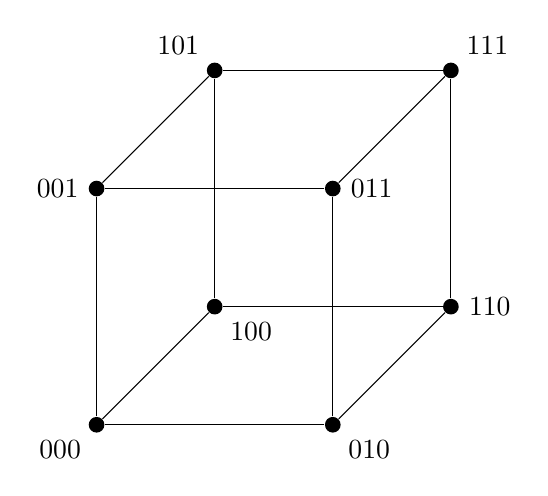
\begin{tikzpicture}[vertex/.style={circle, fill=black, inner sep=2pt}]
    % Outer square: 000(bottom-left), 010(bottom-right), 011(top-right), 001(top-left)
    \node[vertex, label=below left:\(000\)]  (v000) at (0,   0)   {};
    \node[vertex, label=below right:\(010\)] (v010) at (3,   0)   {};
    \node[vertex, label=right:\(011\)] (v011) at (3,   3)   {};
    \node[vertex, label=left:\(001\)]  (v001) at (0,   3)   {};
    % Inner square (offset upper-right): 100, 110, 111, 101
    \node[vertex, label=below right:\(100\)]       (v100) at (1.5, 1.5) {};
    \node[vertex, label=right:\(110\)]        (v110) at (4.5, 1.5) {};
    \node[vertex, label=above right:\(111\)]        (v111) at (4.5, 4.5) {};
    \node[vertex, label=above left:\(101\)]       (v101) at (1.5, 4.5) {};
    % Outer square edges
    \draw (v000)--(v010)--(v011)--(v001)--(v000);
    % Inner square edges
    \draw (v100)--(v110)--(v111)--(v101)--(v100);
    % Connecting edges (differ in MSB)
    \draw (v000)--(v100) (v010)--(v110) (v011)--(v111) (v001)--(v101);
  \end{tikzpicture}
\end{center}

\begin{teorema}{Todo hipercubo es bipartito}{hipercubos_bipartito}
  Para todo \(k>1\), el hipercubo \(Q_k\) es un grafo bipartito.
\end{teorema}

Se establece la bipartición \((X,Y)\) en donde \(X\) contiene a todos los vértices con una cantidad impar de \(1\) y \(Y\) contiene a todos los vértices con una cantidad par de \(1\). Dicho de otra forma, para cada vértice en \(X\), la suma de sus componentes es impar, mientras que para cada vértice en \(Y\), la suma de sus componentes es par:\begin{gather*}
X = \left\{(b_1,\ldots,b_k) \in \{0,1\}^k \quad \Big| \quad \sum_{i=1}^kb_i \equiv 1\mod 2\right\} \\
Y = \left\{(b_1,\ldots,b_k) \in \{0,1\}^k \quad \Big| \quad \sum_{i=1}^kb_i \equiv 0\mod 2\right\}
\end{gather*}Nótese que \(X \cup Y = V\) y que \(X \cap Y = \varnothing\). Hace falta entonces demostrar que todo arco tiene un extremo en \(X\) y otro en \(Y\). Eso es equivalente a demostrar que ningún arco tiene ambos extremos en \(X\) ni ambos extremos en \(Y\).

Para eso, note que dada una tupla binaria, si se cambia únicamente un componente de la tupla binaria, la sumatoria de sus componentes cambia de paridad (i.e., cambia de ser par a ser impar o de ser impar a ser par). Si se cambia un \(1\) por un \(0\), la sumatoria disminuye en \(1\), cambiando de paridad, y si se cambia un \(0\) por un \(1\), la sumatoria aumenta en \(1\), nuevamente cambiando de paridad.

Así pues, no hay ningún par de vértices que estén en el mismo conjunto y sean adyacentes. Para que eso pasara, tendría que ocurrir que dos tuplas binarias con exactamente una coordenada distinta tuvieran una suma de componentes con igual paridad, lo cual no es posible.

Por ende, ningún arco une dos vértices en \(X\) y ningún arco une dos vértices en \(Y\), de forma que efectivamente \((X,Y)\) es una bipartición y \(Q_k\) es bipartito.

\subsection{Grados mínimos para identificar un grafo bipartito conexo}
\label{sec:grados_minimos_para_grafo_bipartito_conexo}

\begin{teorema}{Suma de grados mínimos de bipartición}{suma_grad_min_bip}
  Sea \(G\) un grafo simple bipartito con partición \((X, Y)\) y orden \(n\). Sea \(\delta_X\) el grado mínimo entre los vértices de \(X\) y \(\delta_Y\) el grado mínimo entre los vértices de \(Y\). Si \(\delta_X + \delta_Y > n/2\) entonces \(G\) es conexo.
\end{teorema}

% TODO: Parece que existe una demostración más elegante/sucinta que esta. Buscarla luego.

Considérese un vértice cualquiera \(u \in X\). Se sabe que \(u\) está unido a al menos \(\delta_X\) vértices en \(Y\). Sea \(v\) uno de esos vértices, de forma que \(v\in Y\) y \((u,v) \in E\).

Se sabe que \(\delta_X > n/2 -\delta_Y\) y que \(\delta_X, \delta_Y \in \mathbb{N}\) por ser grados. A partir de eso, se tiene que \[
\delta_X \geq n/2+1-\delta_Y.
\]Por ende, se puede decir que \(u\) está unido a al menos \(n/2+1-\delta_Y\) vértices en \(Y\). Uno de esos vértices es \(v\), que a su vez está unido a al menos \(\delta_Y\) vértices en \(X\). Por ende, \(v\) y \(u\) conforman una componente conexa que tiene como mínimo la siguiente cantidad de vértices: \begin{gather*}
\delta_Y + \left(\frac{n}{2}+1-\delta_Y\right) = \frac{n}{2}+1.
\end{gather*}

Ese raciocinio se puede aplicar a cualquier vértice \(u \in X\), así como a cualquier vértice en \(Y\). Por ende, cada uno de los vértices en \(X\), al igual que cada uno de los vértices en \(Y\), hace parte de una componente conexa con al menos \(n/2+1\) vértices.

Note entonces que no puede ocurrir que dos vértices pertenezcan a componentes conexas distintas. Como cada vértice está en una componente conexa \(C\) donde \(|C| \geq n/2+1\), y el grafo tiene \(n\) vértices en total, debe pasar que cada par de componentes conexas compartan al menos un vértice (si fuesen disyuntas, la suma de vértices sería al menos \(2(n/2+1) = n+2 > n\)).

Por ende, como todas las componentes conexas comparten al menos un vértice, realmente es una gran componente conexa que cubre todo el grafo y se dice que \(G\) es conexo.

% TODO!
% \subsection{Número de acoplamientos perfectos}
% \label{sec:numero_de_acoplamientos_perfectos}

% Hay \(n!\) acoplamientos perfectos en \(K_{n,n}\).

% En \(K_{2n}\),